\documentclass[12pt, letterpaper]{report}

%\usepackage[a4paper, portrait, margin=1in]{geometry}
\usepackage[utf8]{inputenc}
\usepackage[english]{babel}
\usepackage[T1]{fontenc}
\usepackage{concmath} % Text Font
\usepackage{amsmath} % Matrix
\usepackage{parskip}
\usepackage{tabularx} % Manage Tables
\usepackage{makecell} % Manage table cells
\usepackage{fancyhdr} % For Headers and Footers
%\usepackage[htt]{hyphenat} % To solve \textit line break problem
\usepackage{hyperref} % For index and web links
\usepackage[dvipsnames]{xcolor}
\usepackage{tikz} % Graph design
\usepackage{pdflscape} % Page orientation

\usetikzlibrary{positioning}
\usetikzlibrary{calc}
\usetikzlibrary{arrows.meta}

\graphicspath{ {./img/} }

\title{"Control of Mobile Robot" Project}
\author{Colli Stefano, Pagani Mattia, Panelli Erica}
\date{\today}

\pagestyle{fancy}
\fancyhf{}
\rhead{CMR Project}
\lhead{User Manual}
\rfoot{\thepage}

\begin{document}
	
%\maketitle
\begin{titlepage}
	\begin{center}
		
\includegraphics[width=0.6\textwidth]{img/Logo_Politecnico_Milano}
		
		\vspace{4cm}
		
		\huge
		\textbf{Extended project work}
		
		\vspace{0.3cm}
		
		\Large
		A Gazebo car simulator, analysis and comparison with a single-track model
		
		\vspace{1.5cm}
		
		\Large
		\textbf{Colli Stefano, Pagani Mattia, Panelli Erica}
		
		\vfill
		
		\large
		"Control of Mobile Robots" Course
		
		A.A. 2022/2023
	\end{center}
\end{titlepage}

\begin{abstract}
\end{abstract}

\tableofcontents

\newpage

%\section{Gazebo Body Parameters}
%
%\begin{itemize}
%	\item $\mu_0$: friction coefficient of direction 1
%	\item $\mu_1$: friction coefficient of direction 2
%	\item fdir: specify direction of $\mu_0$, direction of $\mu_1$ is perpendicular to this parameter
%	\item $k_p$: stiffness between bodies
%	\item $k_d$: dumping between bodies
%\end{itemize}

\chapter{Notes on Installation and Launch}

\section{Installation}

\subsection{Downloading material}

The project is based on the material of original MIT racecar. That's it, we have generated a new ROS environment copying MIT repository packages. In particular the following packages have been downloaded:

\begin{itemize}
	\item ackermann\_msgs
	\item racecar
	\item racecar\_gazebo
\end{itemize} 

They can be found at the link: \url{https://github.com/mit-racecar}

\subsection{Additional packages to be installed}

To be able to compile the project it is necessary to download two internal ROS packages which will be used by the racecar ones. Launch the following commands:

\begin{verbatim}
sudo apt install ros-noetic-ros-control
sudo apt install ros-noetic-ros-controllers
\end{verbatim}

\noindent Otherwise an error will be thrown when \verb|catkin_make| command is called.

\subsection{Additional modifications}

In some cases, to avoid conflicts, it's required to change Python environment to version 3 in each file of the original packages.
In particular, if Python environment is set to 3, modifications are needed for \verb|joy_teleop.py| file:

\begin{itemize}
	\item Row 277: replace ',' with 'as'
	\item Row 282: replace \verb|iteritems| with \verb|items|
\end{itemize}

\section{Launch}

\subsection{Original Project}

In order to launch original project, once it's compiled following ROS guide, following steps should be followed:

\begin{itemize}
	\item (run) \verb|roscore|
	\item (run) \verb|keyboard_teleop.py|
	\item (run) \verb|racecar_gazebo racecar.tunnel|
\end{itemize}

If there are no errors the user should be able to see the racecar in a Gazebo environment. WASD keys on keyboard produce car moves.

\chapter{General Project Structure}

\section{Catkin Workspace Directories}

\subsection{Original MIT Racecar Packages}

\begin{center}
	\begin{tabularx}{\textwidth}{
			| >{\raggedright\arraybackslash}X
			| >{\arraybackslash}X |
		}
		\hline
		ackermann\_cmd\_mux (racecar folder) & ... \\
		\hline
		ackermann\_msgs & Contains definitions of \textbf{AckermannDrive} and \textbf{AckermannDriveStamped} messages, used by the racecar to compute movements. \\
		\hline
		racecar (racecar folder) & Directory which contains \\
		\hline
		racecar\_control (racecar\_gazebo folder) & Contains launch files to load controllers used to manage the motors of the racecar. Also load nodes which dispatch messages to controllers. \\
		\hline
		racecar\_description (racecar\_gazebo folder) & Contains a description of the racecar, in terms of models, meshes ecc... It will be used by Gazebo to represent it. \\
		\hline
		racecar\_gazebo (racecar\_gazebo folder) & Mainly contains launch scripts used to load all necessary nodes, worlds and other components to open a Gazebo instance with a controllable car. \\
		\hline
	\end{tabularx}
\end{center}

\subsection{Added Packages}

\begin{center}
	\begin{tabularx}{\textwidth}{
			| >{\raggedright\arraybackslash}X
			| >{\raggedright\arraybackslash}X |
		}
		\hline
		car\_control & Contains node which performs the linearization of the nonlinear bycicle \textbf{dynamic} model. It' receives desired velocities from trajectory tracker and sends Ackermann commands to the racecar. \\
		\hline
		car\_kinematic\_control & Contains node which performs the exact linearization of the nonlinear bycicle \textbf{kinematic} model. It' receives desired velocities from trajectory tracker and sends Ackermann commands to the racecar. \\
		\hline
		trajectory\_tracker & Generates (or receives in input) a desired trajectory and actual car positions, than compute desired velocities to be sent to controllers. \\
		\hline
		CarCommandsFr & Interface used to replace inner wheel friction phisical model of ROS with a custom one. \\
		\hline
	\end{tabularx}
\end{center}

\chapter{Original System Introduction}

\chapter{(Our) System Description}

\section{Scheme of the whole system}

\begin{tikzpicture}
\node[
	draw,
	fill=BlueGreen,
	minimum width=2cm,
	minimum height=1.5cm
] (tracker) {Trajectory Tracker};

\node[
	draw,
	fill=BlueGreen,
	minimum width=2cm,
	minimum height=1.5cm,
	right=4cm of tracker
] (refVelocity) {Compute Ref. Velocity};

\node[
	draw,
	fill=Green,
	minimum width=2cm,
	minimum height=1.5cm,
	below=3cm of tracker
] (model) {Model MIT/ODE};

\node[
	draw,
	fill=Yellow,
	minimum width=2cm,
	minimum height=1.5cm,
	below=3cm of refVelocity
] (controller) {Controller};

\draw[-{Triangle[scale=2]}]  (-3, +1/3) --  ($(tracker.west) + (0, +1/3)$)
	node[midway, above]{$x_{ref}$};
	
\draw[-{Triangle[scale=2]}]  (-3, -1/3) --  ($(tracker.west) + (0, -1/3)$)
	node[midway, above]{$y_{ref}$};

% ---

\draw[-{Triangle[scale=2]}] ($(tracker.east) + (0, +1/3)$) -- ($(refVelocity.west) + (0, +1/3)$)
	node[midway, above]{$x_{current}$};
	
\draw[-{Triangle[scale=2]}] ($(tracker.east) + (0, -1/3)$) -- ($(refVelocity.west) + (0, -1/3)$)
	node[midway, above]{$y_{current}$};
	
% ---
	
\draw[-{Triangle[scale=2]}] ($(refVelocity.south) + (-1/2, 0)$) -- ($(controller.north) + (-1/2, 0)$)
	node[midway, left]{$V_{Xp}$};
	
\draw[-{Triangle[scale=2]}] ($(refVelocity.south) + (+1/2, 0)$) -- ($(controller.north) + (+1/2, 0)$)
	node[midway, left]{$V_{Yp}$};

% ---

\draw[-{Triangle[scale=2]}] ($(controller.west) + (0, +1/2)$) -- ($(model.east) + (0, +1/2)$)
	node[midway, above]{$\phi$};
	
\draw[-{Triangle[scale=2]}] ($(controller.west) + (0, 0)$) -- ($(model.east) + (0, 0)$)
	node[midway, above]{$V$};
	
\draw[-{Triangle[scale=2]}] ($(controller.west) + (0, -1/2)$) -- ($(model.east) + (0, -1/2)$)
	node[midway, above]{$\omega$};

% ---

\draw[-{Triangle[scale=2]}] ($(model.north) + (-1/2, 0)$) -- ($(tracker.south) + (-1/2, 0)$)
	node[near end, left]{$x_{in}$}
	node[near start, left]{$x_{out}$};
	
\draw[-{Triangle[scale=2]}] ($(model.north) + (+1/2, 0)$) -- ($(tracker.south) + (+1/2, 0)$)
	node[near end, left]{$y_{in}$}
	node[near start, left]{$y_{out}$};
	
\draw[-{Triangle[scale=2]}] (model.south) |- ++ (0, -1) -| (controller.south)
	node[near start, above]{$\theta_{out}$};

\end{tikzpicture}

\vspace{1cm}

\begin{center}
	\begin{tabularx}{\textwidth}{|l|X|}
		\hline
		\textbf{Symbol} & \textbf{Meaning} \\
		\hline
		$x_{ref}, y_{ref}$ & Ref. position of the trajectory \\
		\hline
		$V_{Xp}, V_{Yp}$ & Required velocities of the point. They will be imposed by controller\\
		\hline
		$\phi$ & Steer degree of rotation \\
		\hline
		$V$ & Vector velocity \\
		\hline
		$\omega$ & Steer speed of rotation \\
		\hline
		$\theta_{out}$ & Car pose: rotation around center axis\\
		\hline
		$x_{out}, y_{out}$ & Car pose: x, y \\
		\hline
	\end{tabularx}
\end{center}

\vspace{1cm}

Note that "trajectory tracker" generated trajectories are hard-coded, even if $x_{ref}$ and $y_{ref}$ are shown as input parameters. The user can select the trajectory using YAML configuration file (which will be explained in the relative section).

\section{Topics}

\subsection{Scheme of topic publications/subscriptions}

\subsubsection{ROS Friction Model}

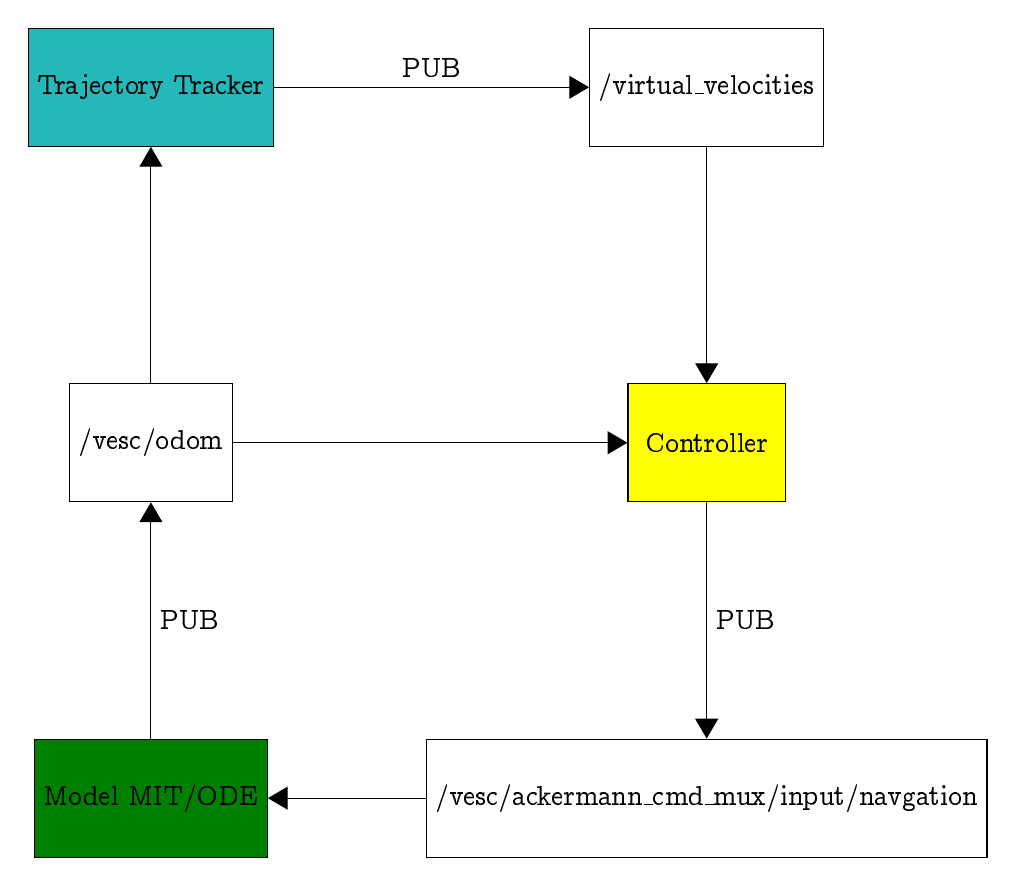
\begin{tikzpicture}
	
\node[
	draw,
	fill=BlueGreen,
	minimum width=2cm,
	minimum height=1.5cm
] (tracker) {Trajectory Tracker};

\node[
	draw,
	fill=White,
	minimum width=2cm,
	minimum height=1.5cm,
	right=4cm of tracker
] (virtualVel) {/virtual\_velocities};

\node[
	draw,
	fill=White,
	minimum width=2cm,
	minimum height=1.5cm,
	below=3cm of tracker
] (odom) {/vesc/odom};

\node[
	draw,
	fill=Yellow,
	minimum width=2cm,
	minimum height=1.5cm,
	below=3cm of virtualVel
] (controller) {Controller};

\node[
	draw,
	fill=Green,
	minimum width=2cm,
	minimum height=1.5cm,
	below=3cm of odom
] (model) {Model MIT/ODE};

\node[
	draw,
	fill=White,
	minimum width=2cm,
	minimum height=1.5cm,
	below=3cm of controller
] (ackermanCmd) {/vesc/ackermann\_cmd\_mux/input/navgation};

% ---

\draw[-{Triangle[scale=2]}] (tracker.east) -- (virtualVel.west)
	node[midway, above]{PUB};
	
\draw[-{Triangle[scale=2]}] (virtualVel.south) -- (controller.north)
	node[midway, right]{};
	
\draw[-{Triangle[scale=2]}] (controller.south) -- (ackermanCmd.north)
	node[midway, right]{PUB};
	
\draw[-{Triangle[scale=2]}] (ackermanCmd.west) -- (model.east)
	node[midway, above]{};
	
\draw[-{Triangle[scale=2]}] (model.north) -- (odom.south)
	node[midway, right]{PUB};
	
\draw[-{Triangle[scale=2]}] (odom.north) -- (tracker.south)
	node[midway, right]{};
	
\draw[-{Triangle[scale=2]}] (odom.east) -- (controller.west)
	node[midway, above]{};

\end{tikzpicture}

\subsubsection{Custom Friction Model}

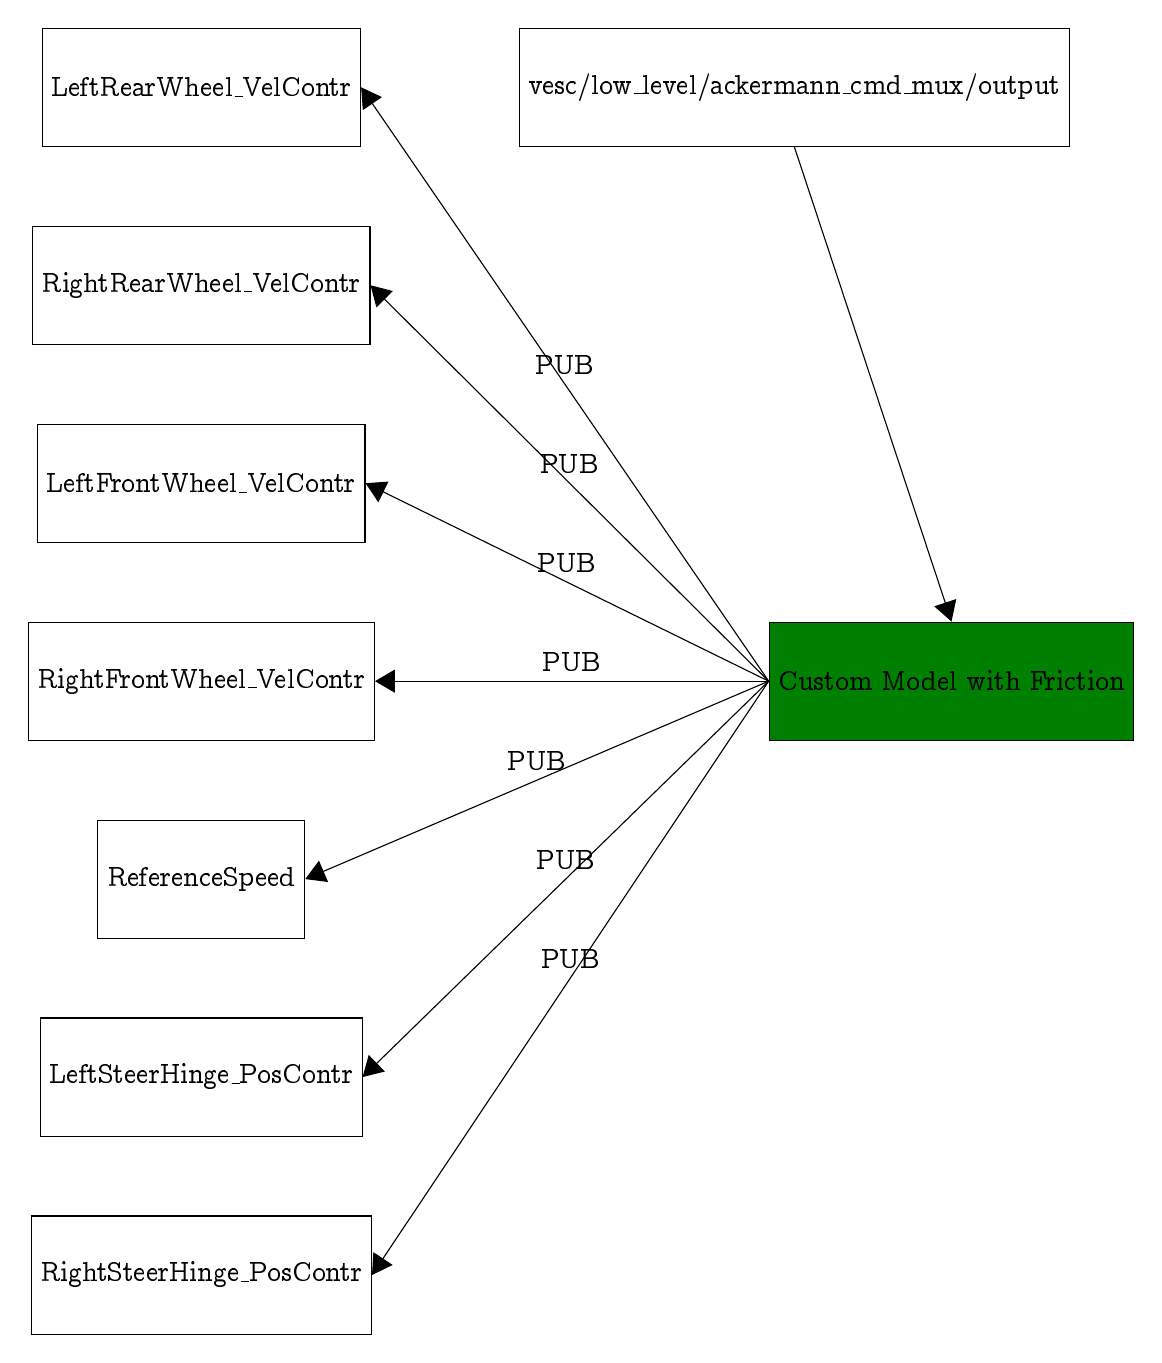
\begin{tikzpicture}
	\node[
	draw,
	fill=White,
	minimum width=2cm,
	minimum height=1.5cm
	] (LRW-VelContr) {LeftRearWheel\_VelContr};
	
	% ---
	
	\node[
	draw,
	fill=White,
	minimum width=2cm,
	minimum height=1.5cm,
	right=2cm of LRW-VelContr
	] (AckermannCmd) {vesc/low\_level/ackermann\_cmd\_mux/output};
	
	% ---
	
	\node[
	draw,
	fill=White,
	minimum width=2cm,
	minimum height=1.5cm,
	below=1cm of LRW-VelContr
	] (RRW-VelContr) {RightRearWheel\_VelContr};
	
	\node[
	draw,
	fill=White,
	minimum width=2cm,
	minimum height=1.5cm,
	below=1cm of RRW-VelContr
	] (LFW-VelContr) {LeftFrontWheel\_VelContr};
	
	\node[
	draw,
	fill=White,
	minimum width=2cm,
	minimum height=1.5cm,
	below=1cm of LFW-VelContr
	] (RFW-VelContr) {RightFrontWheel\_VelContr};
	
	% ---
	
	\node[
	draw,
	fill=Green,
	minimum width=2cm,
	minimum height=1.5cm,
	right=5cm of RFW-VelContr
	] (Model) {Custom Model with Friction};
	
	% ---
	
	\node[
	draw,
	fill=White,
	minimum width=2cm,
	minimum height=1.5cm,
	below=1cm of RFW-VelContr
	] (RefSpeed) {ReferenceSpeed};
	
	\node[
	draw,
	fill=White,
	minimum width=2cm,
	minimum height=1.5cm,
	below=1cm of RefSpeed
	] (LSH-PosContr) {LeftSteerHinge\_PosContr};
	
	\node[
	draw,
	fill=White,
	minimum width=2cm,
	minimum height=1.5cm,
	below=1cm of LSH-PosContr
	] (RSH-PosContr) {RightSteerHinge\_PosContr};
	
	\draw[-{Triangle[scale=2]}] (AckermannCmd.south) -- (Model.north)
	node[midway, above]{};
	
	\draw[-{Triangle[scale=2]}] (Model.west) -- (LRW-VelContr.east)
	node[midway, above]{PUB};
	
	\draw[-{Triangle[scale=2]}] (Model.west) -- (RRW-VelContr.east)
	node[midway, above]{PUB};
	
	\draw[-{Triangle[scale=2]}] (Model.west) -- (LFW-VelContr.east)
	node[midway, above]{PUB};
	
	\draw[-{Triangle[scale=2]}] (Model.west) -- (RFW-VelContr.east)
	node[midway, above]{PUB};
	
	\draw[-{Triangle[scale=2]}] (Model.west) -- (RefSpeed.east)
	node[midway, above]{PUB};
	
	\draw[-{Triangle[scale=2]}] (Model.west) -- (LSH-PosContr.east)
	node[midway, above]{PUB};
	
	\draw[-{Triangle[scale=2]}] (Model.west) -- (RSH-PosContr.east)
	node[midway, above]{PUB};	
\end{tikzpicture}

\subsection{Topics meaning}

\subsubsection{Common Topics}

\begin{center}
	\begin{tabularx}{\textwidth}{
			| >{\raggedright\arraybackslash}X
			| >{\raggedright\arraybackslash}X |
		}
		\hline
		/virtual\_velocities & Used by "trajectory tracker" to publish desired velocity components. These are read by controller in order to perform linearization and compute instructions for the model. \\
		\hline
		\makecell[lt]{/vesc/ackermann\_cmd\_mux \\ /input/navgation} & Contains AckermannDriveStamped messages sent by controller. These messages contains information for the racecar, about velocity and steering. \\
		\hline
		/vesc/odom & The model uses this topic to publish odometry information of the racecar (position and orientation). These data are used both by tracker and controller. The first one compute differences between actual car position and desired position imposed by trajectory. The last one reads z-axis orientation useful to perform linearization. \\
		\hline
	\end{tabularx}
\end{center}

There is another topic in which "trajectory tracker" publish, the \textit{/reference\_trajectory}. This is used to read trajectory information to perform debug and register data for analysis.

\vspace{1cm}

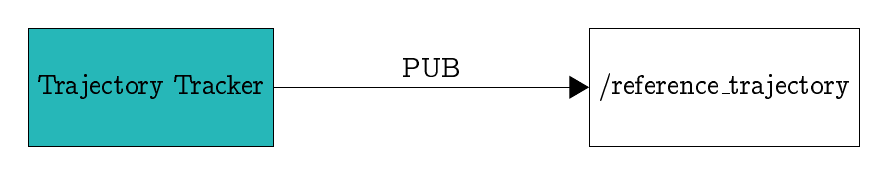
\begin{tikzpicture}
	
\node[
	draw,
	fill=BlueGreen,
	minimum width=2cm,
	minimum height=1.5cm
] (tracker) {Trajectory Tracker};

\node[
	draw,
	fill=White,
	minimum width=2cm,
	minimum height=1.5cm,
	right=4cm of tracker
] (reference) {/reference\_trajectory};

\draw[-{Triangle[scale=2]}] (tracker.east) -- (reference.west)
	node[midway, above]{PUB};

\end{tikzpicture}

\subsubsection{Specific Topics}

\begin{center}
	\begin{tabularx}{\textwidth}{
			| >{\raggedright\arraybackslash}X
			| >{\raggedright\arraybackslash}X |
		}
		\hline
		\makecell[lt]{/vesc/low\_level/ \\ ackermann\_cmd\_mux/output} & xyz \\
		\hline
		\makecell[lt]{/racecar/ \\ left\_rear\_wheel \\ \_velocity\_controller/command} & xyz \\
		\hline
		\makecell[lt]{/racecar/ \\ right\_rear\_wheel \\ \_velocity\_controller/command} & xyz \\
		\hline
		\makecell[lt]{/racecar/ \\ left\_front\_wheel \\ \_velocity\_controller/command} & xyz \\
		\hline
		\makecell[lt]{/racecar/ \\ right\_front\_wheel \\ \_velocity\_controller/command} & xyz \\
		\hline
		\makecell[lt]{/reference\_speed} & xyz \\
		\hline
		\makecell[lt]{/racecar/ \\ left\_steering\_hinge \\ \_position\_controller/command} & xyz \\
		\hline
		\makecell[lt]{/racecar/ \\ right\_steering\_hinge \\ \_position\_controller/command} & xyz \\
		\hline
	\end{tabularx}
\end{center}

\chapter{Detailed Package Description}

\section{Package (original) ackermann\_msgs}
\section{Package (original) racecar}
\section{Package (original) racecar\_gazebo}

\section{Package car\_control}

\subsection{Intro}

Even if this package is not used, it's correct to do a description of the objective it should have reached.

The aim was to implement a dynamic controller, which perform exact linearization of the nonlinear bicycle dynamic model. To do this it needs more parameter respect to the kinematic one.

In addition, we put a scheme (\ref{fig:dynamic_model}) of the principal parameters and variables  used for linearization.

\begin{figure}[h]
	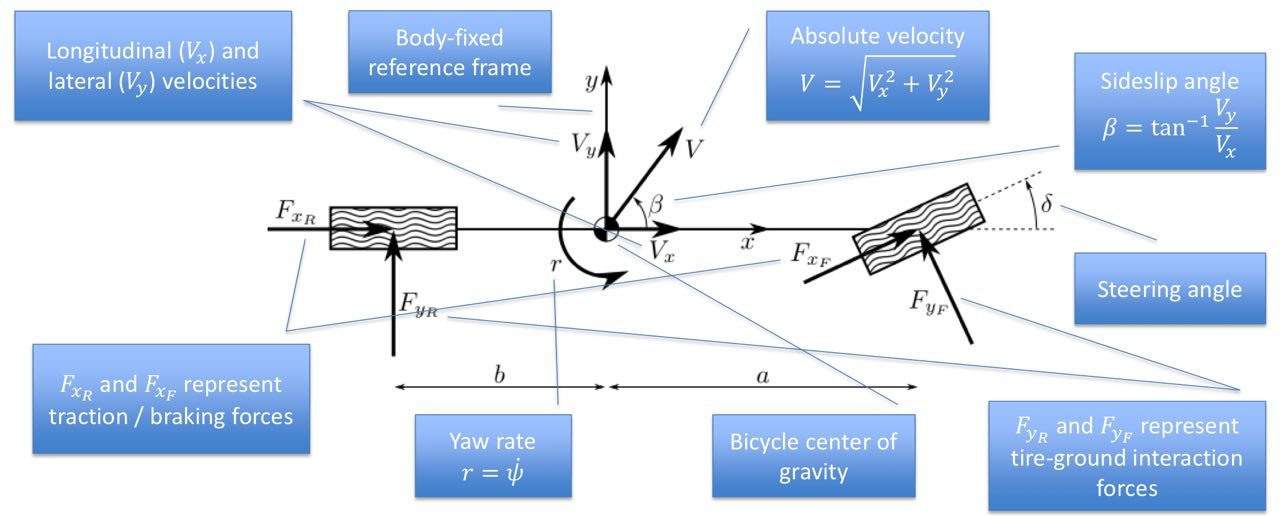
\includegraphics[scale=0.3]{dynamic_model}
	\caption{dynamic model with main parameters and variables}
	\label{fig:dynamic_model}
\end{figure}

\subsection{Configuration}

\begin{center}
	\begin{tabularx}{\textwidth}{
			| >{\raggedright\arraybackslash}X
			| >{\arraybackslash}X |
		}
		\hline
		\multicolumn{2}{|c|}{\textbf{Input values}} \\
		\hline
		$Vp_x$ & Point velocity x \\
		\hline
		$Vp_y$ & Point velocity y \\
		\hline
		$\psi$ & Yaw\footnote{In the System Scheme, this is represented by $\theta_{out}$} \\
		\hline
		$\dot{\psi}$ & Yaw rate\footnote{In the System Scheme, this is \textbf{not} represented (as we have used, for tests, only the kinematic model)} \\
		\hline
	\end{tabularx}
	
	\vspace{0.5cm}
	
	\begin{tabularx}{\textwidth}{
			| >{\raggedright\arraybackslash}X
			| >{\arraybackslash}X |
		}
		\hline
		\multicolumn{2}{|c|}{\textbf{Model parameters}} \\
		\hline
		$C_f$, $C_r$ & Viscuous friction coefficients \\
		\hline
		a, b & Distance between wheels center and Center of Gravity \\		
		\hline
		$M$ & Vehicle mass \\
		\hline
		$\epsilon$ & Distance between Center of Gravity and a point $P$, along the velocity vector. Linearization is done around point P. This parameter should be chosen empirically \\
		\hline
	\end{tabularx}
	
	\vspace{0.5cm}
	
	\begin{tabularx}{\textwidth}{
			| >{\raggedright\arraybackslash}X
			| >{\arraybackslash}X |
		}
		\hline
		\multicolumn{2}{|c|}{\textbf{Intermediate computed values}} \\
		\hline
		$\beta$ & Sideslip angle: $\tan^{-1}\left(\frac{Vp_y}{Vp_x}\right)$ \\
		\hline
	\end{tabularx}
	
	\vspace{0.5cm}
	
	\begin{tabularx}{\textwidth}{
			| >{\raggedright\arraybackslash}X
			| >{\arraybackslash}X |
		}
		\hline
		\multicolumn{2}{|c|}{\textbf{Output values}} \\
		\hline
		$V$ & Point absolute velocity \\
		\hline
		$\delta$ & Steering angle \\
		\hline
		$\omega$ & Steering speed \\
		\hline
	\end{tabularx}
\end{center}

\subsection{Launch}

There is a lunch file which \textbf{should be used to execute the node}. This contains also information about debugging level and loads configuration file.

\subsection{Node car\_control}

\[
\beta = \tan^{-1}\left(\frac{Vp_y}{Vp_x}\right)
\]
\[
\delta = \frac{MV}{C_f}\omega + \frac{C_f + C_r}{C_f}\beta - \frac{bC_r - aC_f}{C_f}\frac{\dot{\psi}}{V}
\]
\[
\begin{bmatrix}
	V \\
	\omega
\end{bmatrix}
=
\begin{bmatrix}
	\cos(\beta + \psi) & \sin(\beta + \omega) \\
	-\frac{\sin(\beta + \psi)}{\epsilon} & \frac{\cos(\beta + \psi)}{\epsilon} \\
\end{bmatrix}
\begin{bmatrix}
	Vp_x \\
	Vp_y
\end{bmatrix}
\]

\section{Package car\_kinematic\_control}

\subsection{Intro}

Before starting the explanation, we add a brief high level description of Quaternions, which are used in messages to represent orientations. Even a distinction between pose and position is done.

\textbf{Quaternion}: a different way to describe the orientation of a frame only. It's an alternative to Yaw, Pitch and Roll. A quaternion has four parameters: x, y, z, w. Pay attention, they are NOT a position vector.

\textbf{Position}: position of the robot in a 3D space.

\textbf{Pose}: position (3 DOF) + orientation (3 DOF).

In conclusion the pose has 6 D.O.F. which are: x, y, z, roll, pitch, yaw. Euler angles can be converted to quaternions, which are better. Transformation functions of ROS can do this conversion and the reverse one.

In addition, we put a scheme (\ref{fig:bicycle_vehicle}) of the principal parameters and variables  used for linearization.

\begin{figure}[h]
	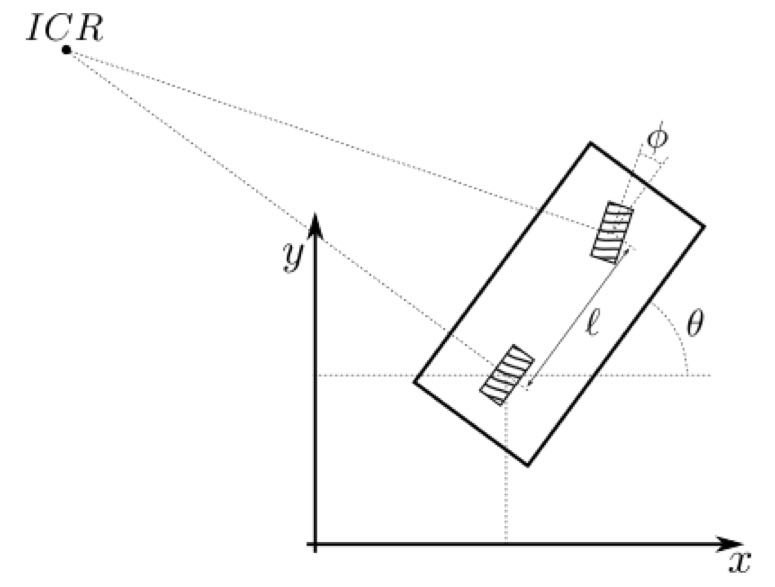
\includegraphics[scale=0.4]{kinematic_model}
	\caption{bicycle vehicle with main parameters and variables}
	\label{fig:bicycle_vehicle}
\end{figure}

\subsection{Configuration}

In the package there is a configuration file, containing: the parameter L, which represents distance between rear and front wheels; the parameter $\epsilon$, the distance between Center of Gravity and a point $P$, along the velocity vector. Linearization is done around point P. This parameter should be chosen empirically.
 
Both are used in the linearization.

\subsection{Launch}

There is a lunch file which \textbf{should be used to execute the node}. This contains also information about debugging level and loads configuration file.

\subsection{Node car\_kin\_controller}

\textbf{Node requirements}: distance between rear and front wheels as parameter.

The node has two callbacks:

\begin{itemize}
	\item One used to retrieve desired velocities of the point. These velocities are computed by trajectory tracker and published in \verb|/virtual_velocities| topic, subscribed by the controller node.
	\item One used to retrieve the orientation of the car around z axis. This is done reading from \verb|/vesc/odom|. The information retrieved are in the form of a quaternion and are converted into roll, pitch and yaw. Yaw is taken. In addition, even the speed around z axis is read (\verb|twist.angular.z|).
\end{itemize}

The node perform an exact linearization of the nonlinear bicycle cinematic model. The change of coordinates is applied as follows:

\[
V = V_{Xp}cos(\theta) + V_{Yp}sin(\theta)
\]

\[
\phi = \arctan\left(\frac{l}{\epsilon} \frac{ V_{Yp}cos(\theta) - V_{Xp}sin(\theta) }{ V_{Xp}cos(\theta) + V_{Yp}sin(\theta) }\right)
\]

Where 

\begin{itemize}
	\item $l$ is the distance between rear and front wheels
	\item $\epsilon$ is the distance between Center of Gravity and a point $P$
	\item $V_{Xp}$ and $V_{Yp}$ are the desired point velocities
	\item $\theta$ is the car orientation around z-axis
	\item $\phi$ is the steering angle
	\item $V$ is the driving velocity of the front wheel
\end{itemize}

In addition, the program compute the steering speed as $\omega = \frac{V}{l}\tan(\phi)$. This value is not used in the construction of the message because it's ignored by the model.

Once the linearization is performed an \verb|AckermannDriveStamped| message is built, containing $V$ and $\phi$. This message is published on \\ \verb|/vesc/ackermann_cmd_mux/input/navigation| topic, which is read by the model to make the car move. Linearization and command sending operations are repeated in a loop, which is the core of the node.

\section{Package trajectoy\_tracker}

\subsection{Configuration}

In the YAML configuration file are present many parameters which are used in the node.

\begin{center}
	\begin{tabularx}{\textwidth}{
			| >{\raggedright\arraybackslash}X
			| >{\arraybackslash}X |
		}
		\hline
		\multicolumn{2}{|c|}{\textbf{Node configuration parameters}} \\
		\hline
		trajectory\_type & Desired trajectory (0 = linear; 1 = parabolic; 2 = circular; 3 = eight shape; 4 = cycloidal; 5 = fixed point) \\
		\hline
	\end{tabularx}
	
	\vspace{2em}
	
	\begin{tabularx}{\textwidth}{
			| >{\raggedright\arraybackslash}X
			| >{\arraybackslash}X |
		}
		\hline
		\multicolumn{2}{|>{\centering}X|}{\textbf{Linear trajectory parameters. The trajectory is parallel to the direction vector (a\_coeff, b\_coeff)}} \\
		\hline
		a\_coeff & \\          
		\hline 
		b\_coeff & \\     
		\hline        
	\end{tabularx}
	
	\vspace{2em}
	
	\begin{tabularx}{\textwidth}{
			| >{\raggedright\arraybackslash}X
			| >{\arraybackslash}X |
		}
		\hline
		\multicolumn{2}{|c|}{\textbf{Parabolic trajectory parameters}} \\
		\hline
		parabola\_convexity & Convexity a of the parabola having equation $y = ax^2$ \\ 
		\hline
	\end{tabularx}
	
	\vspace{2em}
	
	\begin{tabularx}{\textwidth}{
			| >{\raggedright\arraybackslash}X
			| >{\arraybackslash}X |
		}
		\hline
		\multicolumn{2}{|c|}{\textbf{Circular trajectory parameters}} \\
		\hline
		$R$ & Radius of the circle described by the trajectory \\
		\hline
		$W$ & Angular speed for the lap ($W = 2\pi/T$, where $T$ is the time duration of each lap) \\
		\hline
	\end{tabularx}
	
	\vspace{2em}
	
	\begin{tabularx}{\textwidth}{
			| >{\raggedright\arraybackslash}X
			| >{\arraybackslash}X |
		}
		\hline
		\multicolumn{2}{|c|}{\textbf{Eight-shape trajectory parameters}} \\
		\hline
		$a$ & Trajectory amplitute (the eight-shape goes from $-a$ to $a$) \\
		\hline
		$w$ & Angular speed for the lap ($w = 2\pi/T$, where $T$ is the time duration of each lap) \\
		\hline
	\end{tabularx}
	
	\vspace{2em}
	
	\begin{tabularx}{\textwidth}{
			| >{\raggedright\arraybackslash}X
			| >{\arraybackslash}X |
		}
		\hline
		\multicolumn{2}{|c|}{\textbf{Cycloidal trajectory parameter}} \\
		\hline
		cycloid\_radius & Radius of the wheel describing the cycloid \\
		\hline
	\end{tabularx}
	
	\vspace{2em}
	
	\begin{tabularx}{\textwidth}{
			| >{\raggedright\arraybackslash}X
			| >{\arraybackslash}X |
		}
		\hline
		\multicolumn{2}{|c|}{\textbf{Controller parameters}} \\
		\hline
		$Kp$ & Proportional gain \\
		\hline
		$Ki$ & Integral gain \\
		\hline
		$Kd$ & Derivative gain \\
		\hline
		$FFWD$ & Use velocity feedforward (1 = feedforward used; 0 = feedforward NOT used) \\
		\hline
	\end{tabularx}
	
	\vspace{2em}
	
	\begin{tabularx}{\textwidth}{
			| >{\raggedright\arraybackslash}X
			| >{\arraybackslash}X |
		}
		\hline
		\multicolumn{2}{|c|}{\textbf{Robot parameters}} \\
		\hline
		$PL_{distance}$ & Distance from the odometric centre of the robot to the selected point $P$ \\
		\hline
	\end{tabularx}
\end{center}

\subsection{Node trajectory\_tracker}

The main loop executes three actions:

\begin{enumerate}
	\item Computation of reference point for the desired trajectory
	\item Translation of trajectory point from point L to point P % ??? ask
	\item Computation of control action as virtual velocities
\end{enumerate}

\begin{center}
	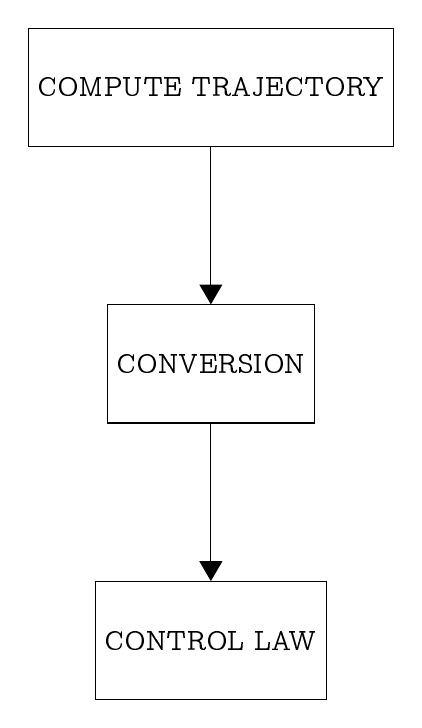
\begin{tikzpicture}
		
	\node[
		draw,
		fill=White,
		minimum width=2cm,
		minimum height=1.5cm
	] (computeTrajectory) {COMPUTE TRAJECTORY};
	
	\node[
		draw,
		fill=White,
		minimum width=2cm,
		minimum height=1.5cm,
		below=2cm of computeTrajectory
	] (conversion) {CONVERSION};
	
	\node[
		draw,
		fill=White,
		minimum width=2cm,
		minimum height=1.5cm,
		below=2cm of conversion
	] (controlLaw) {CONTROL LAW};
	
	\draw[-{Triangle[scale=2]}] (computeTrajectory.south) -- (conversion.north)
		node[midway, right]{};
	
	\draw[-{Triangle[scale=2]}] (conversion.south) -- (controlLaw.north)
		node[midway, right]{};
		
	\end{tikzpicture}
\end{center}

\subsubsection{Compute Trajectory}

\[
t = t_{new} - t_{initial}
\]

% ---

\underline{Linear}

\textit{a\_coeff} in configuration parameters is indicated as $a_{circle}$. 

\textit{b\_coeff} in configuration parameters is indicated as $b_{circle}$.

\[
X_{ref} = a_{circle}t
\]
\[
dx_{ref} = a_{circle}
\]

\[
Y_{ref} = b_{circle}t
\]
\[
dy_{ref} = b_{circle}
\]

% ---

\underline{Parabolic}

PC := Parabola Convexity

\[
X_{ref} = t
\]
\[
dx_{ref} = 1
\]

\[
Y_{ref} = PC \cdot \cos(wt)^2
\]
\[
dy_{ref} = 2 \cdot PC \cdot t
\]

% ---

\underline{Circle}

In parameters file parameter \textit{W} is uppercase.

\[
X_{ref} = R\cos(Wt)
\]
\[
dx_{ref} = -WR\sin(Wt)
\]

\[
Y_{ref} = R\sin(Wt)
\]
\[
dy_{ref} = WR\cos(Wt)
\]

% ---

\underline{Eight}

In parameters file parameter \textit{w} is lowercase.

\[
X_{ref} = a\sin(wt)
\]
\[
dx_{ref} = wa\cos(wt)
\]

\[
Y_{ref} = a\sin(wt)\cos(wt)
\]
\[
dy_{ref} = wa(\cos(wt)^2 - \sin(wt)^2)
\]

% ---

\underline{Cycloidal}

CR := Cycloid Radius

\[
X_{ref} = CR(t - \sin(t))
\]
\[
dx_{ref} = CR - \cos(t)
\]

\[
Y_{ref} = CR(1 - \cos(t))
\]
\[
dy_{ref} = \sin(t)
\]

\subsubsection{Conversion}

\[
Xp_{ref} = X_{ref} + PL_{distance} \cdot \cos(\theta)
\]
\[
Yp_{ref} = Y_{ref} + PL_{distance} \cdot \sin(\theta)
\]

\subsubsection{Control Law}

Compute position error

\[
Xp_{err} = Xp_{ref} - Xp
\]
\[
Yp_{err} = Yp_{ref} - Yp
\]

% ---

Difference between current time and initial one

\[
\Delta T = T_{new} - T
\]

% ---

Compute integral term

\[
X_{int} = X_{int} + Xp_{err} \cdot \Delta T
\]
\[
Y_{int} = Y_{int} + Yp_{err} \cdot \Delta T
\]

% ---

Compute derivative term

\[
X_{der} = (Xp_{err} - Xp_{err\_old}) / \Delta T
\]
\[
Y_{der} = (Yp_{err} - Yp_{err\_old}) / \Delta T
\]

% ---

PI + FFWD controller 

\[
V_{Xp} = FFWD \cdot dx_{ref} + K_p \cdot Xp_{err} + K_i \cdot X_{int} + K_d \cdot X_{der}
\]
\[
V_{Yp} = FFWD \cdot dy_{ref} + K_p \cdot Yp_{err} + K_i \cdot Y_{int} + K_d \cdot Y_{der}
\]

\subsection{Choiche of PID controller and parameters}

\section{Package CarCommndsFr}

\subsection{Intro}

\subsection{Configuration}

\begin{center}
	\begin{tabularx}{\textwidth}{
			| >{\raggedright\arraybackslash}X
			| >{\arraybackslash}X |
		}
		\hline
		\multicolumn{2}{|c|}{\textbf{Surface Parameters}} \\
		\hline
		surface\_type & Select surface type among 1:DRY, 2:WET, 3:SNOW, 4:ICE, 5:CUSTOM (parameters calculated with racecar values) \\
		\hline
	\end{tabularx}
\end{center}

\subsection{Launch}

\subsection{Node car\_commands\_fr}

\subsubsection{Compute surface type}

Values are assigned to coefficients depending on the chosen ground type.

\begin{center}
	\begin{tabularx}{\textwidth}{|X|X|X|X|X|X|X|}
		\hline
		 & $B_x$ & $B_y$ & $C_x$ & $C_y$ & $D$ & $E$ \\
		\hline
		Dry & 10 & 10 & 1.9 & 1.9 & 1 & 0.97 \\
		\hline
		Wet & 12 & 12 & 2.3 & 2.3 & 0.82 & 1 \\
		\hline
		Snow & 5 & 5 & 2 & 2 & 0.3 & 1 \\
		\hline
		Ice & 4 & 4 & 2 & 2 & 0.1 & 1 \\
		\hline
		Custom & 0.21 & 0.017 & 1.65 & 1.3 & -548 & 0.2 \\
		\hline
	\end{tabularx}
\end{center}

\subsubsection{Compute desired speed}

$S$ = slip

$V$ = |speed|

$R_w$ = wheel radius 

$M$ = mass

Longitudinal Slip
\[
\omega = \frac{V}{R_w}
\]
\textcolor{red}{Sempre 0?}
\[
S_{long} = \frac{V - R_w\omega}{V}
\]
Lateral Slip
\[
S_{lat} = \arctan\left(\frac{V_y}{V_x}\right)
\]
Acceleration

Pacejka Magic Formula
\[
y(x) = D\sin\{C\arctan[Bx - E(Bx - \arctan(Bx))]\}
\]
\[
a_{long} = \frac{y(S_{long})}{M}
\]
\[
a_{lat} = \frac{y(S_{lat})}{M}
\]
\[
a = \sqrt[2]{a_{long}^2 + a_{lat}^2}
\]
\[
V_{desired} = \frac{\left(V + a\left(\frac{1}{100}\right)\right)}{0.1}
\]

\appendix

\chapter{launch package inclusion}

\begin{landscape}
	
	\usetikzlibrary{arrows.meta}
	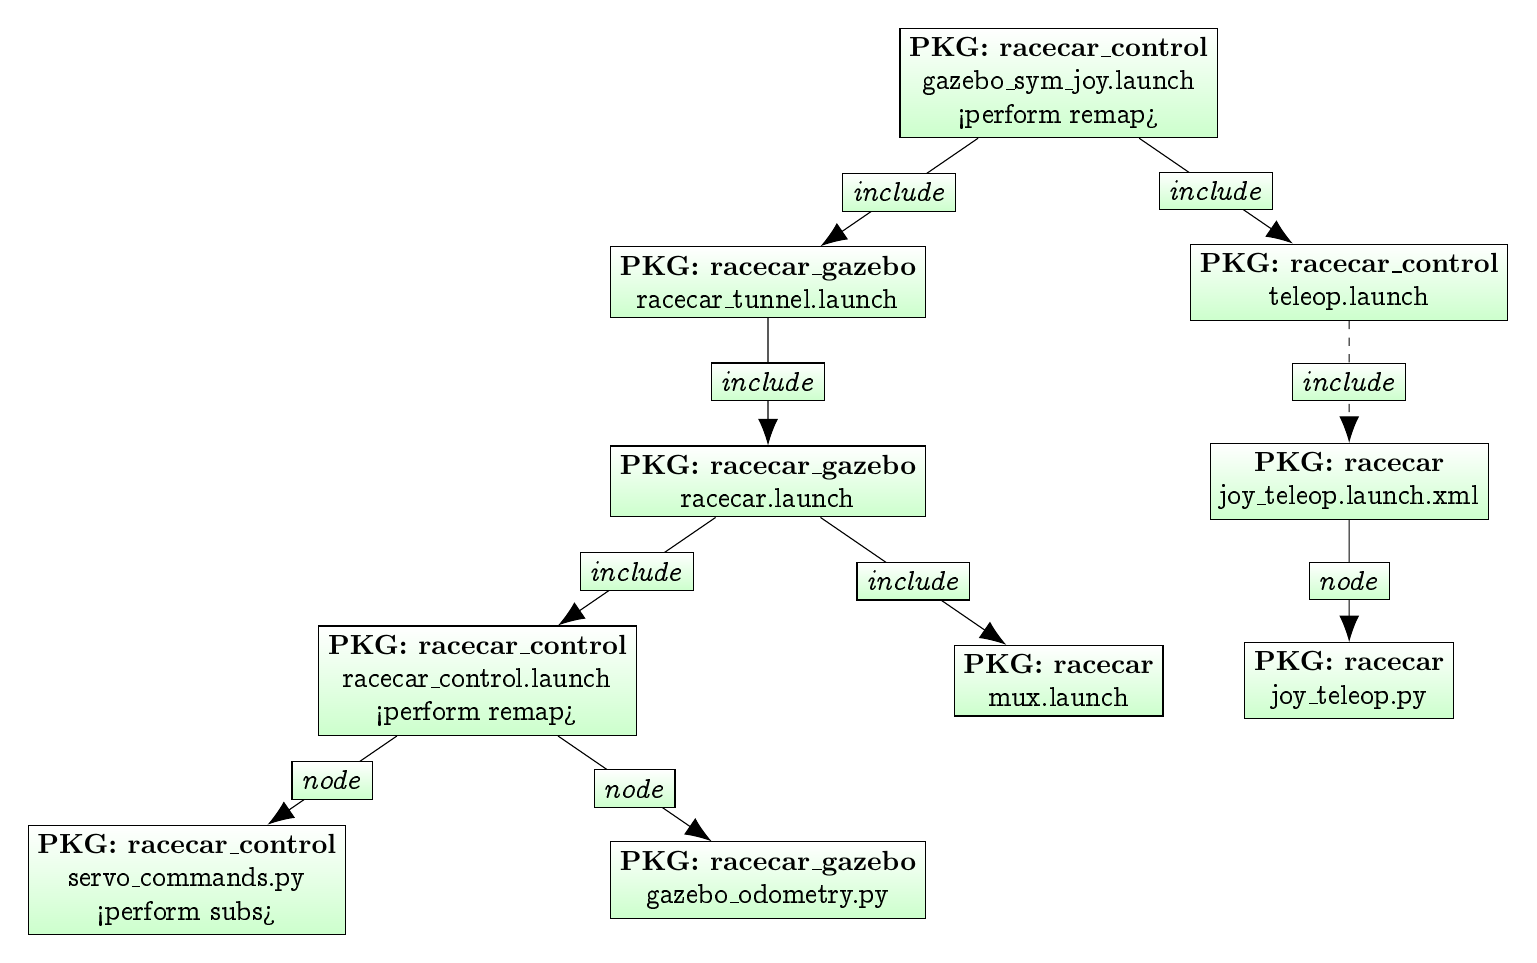
\begin{tikzpicture}[
		level/.style={level distance=7.2em, sibling distance=21em},
		every node/.style = {
			shape=rectangle, 
			solid,
			draw, 
			align=center,
			top color=white, 
			bottom color=green!20
		},
		norm/.style={edge from parent/.style={-{Latex[scale=2]}, solid, draw}},
		emph/.style={edge from parent/.style={-{Latex[scale=2]}, dashed, draw}}
		]
		\node {\textbf{PKG: racecar\_control} \\ gazebo\_sym\_joy.launch \\ <perform remap>}
		child [norm] { node {\textbf{PKG: racecar\_gazebo} \\ racecar\_tunnel.launch} 
			child [norm] { node {\textbf{PKG: racecar\_gazebo} \\ racecar.launch} 
				child [norm] { node {\textbf{PKG: racecar\_control} \\ racecar\_control.launch \\ <perform remap>} 
					child [norm] { node {\textbf{PKG: racecar\_control} \\ servo\_commands.py \\ <perform subs>} edge from parent node {\textit{node}} }
					child [norm] { node {\textbf{PKG: racecar\_gazebo} \\ gazebo\_odometry.py} edge from parent node {\textit{node}} }
					edge from parent node {\textit{include}}
				}
				child [norm] { node {\textbf{PKG: racecar} \\ mux.launch} edge from parent node {\textit{include}} }
				edge from parent node {\textit{include}}
			} 
			edge from parent node {\textit{include}}
		}
		child [norm] { node {\textbf{PKG: racecar\_control} \\ teleop.launch} 
			child [emph] { node {\textbf{PKG: racecar} \\ joy\_teleop.launch.xml} 
				child [norm] { node {\textbf{PKG: racecar} \\ joy\_teleop.py} edge from parent node {\textit{node}} }
				edge from parent node {\textit{include}}
			}
			edge from parent node {\textit{include}}
		};
	\end{tikzpicture}
	
	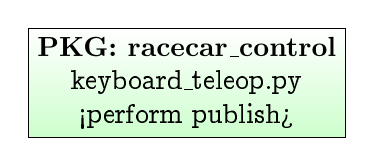
\begin{tikzpicture}[
		sibling distance=18em,
		every node/.style = {
			shape=rectangle, 
			draw, 
			align=center,
			top color=white, 
			bottom color=green!20
		},
		edge from parent/.style= {
			draw,
			-latex
		}
		]
		\node {\textbf{PKG: racecar\_control} \\ keyboard\_teleop.py \\ <perform publish>};
	\end{tikzpicture}
	
\end{landscape}

\begin{center}
	\begin{tabularx}{\linewidth}{|X|X|X|}
		\hline
		\textbf{Package} & \textbf{File} & \textbf{Remap} \\
		\hline
		racecar & joy\_teleop.launch.xml & (none) \\
		\hline
		racecar & joy\_teleop.py & (none) \\
		\hline
		racecar & mux.launch & (none) \\
		\hline
		racecar\_control & gazebo\_sim\_joy.launch & \parbox[t]{5cm}{\raggedright \textcolor{Green}{REMAP \\ /ackermann\_cmd\_ \\ mux/input/teleop \\ TO \\ /racecar/ackermann\_ \\ cmd\_mux/input/teleop}} \\
		\hline
		racecar\_control & teleop.launch & (none) \\
		\hline
		racecar\_control & racecar\_control.launch & \parbox[t]{5cm}{\raggedright \textcolor{Green}{REMAP \\ /racecar/ack/output \\ TO \\ /vesc/low\_level/ \\ ack/output}} \\
		\hline
		racecar\_control & servo\_commands.py & \parbox[t]{5cm}{\raggedright \textcolor{Green}{SUBSCRIBE \\ /racecar/ackermann\_ \\ cmd\_mux/output}} \\
		\hline
		racecar\_control & keybpard\_teleop.py & \parbox[t]{5cm}{\raggedright \textcolor{Green}{PUBLISH \\ /vesc/achermann\_ \\ cmd\_mux/input/teleop}} \\
		\hline
		racecar\_gazebo & racecar\_tunnel.launch & (none) \\
		\hline
		racecar\_gazebo & racecar.launch & (none) \\
		\hline
		racecar\_gazebo & gazebo\_odometry.py & (none) \\
		\hline
	\end{tabularx}
\end{center}

\end{document}